\documentclass{article} % For LaTeX2e
\usepackage{nips15submit_e,times}
\usepackage{hyperref}
\usepackage{url}
\usepackage{amsmath}
\usepackage{graphicx}
%\documentstyle[nips14submit_09,times,art10]{article} % For LaTeX 2.09


\title{Implementation and Analysis of Random Forests}


\author{
Jae Lee\\
School of Computing Science\\
Simon Fraser University\\
Burnaby BC V5A 1S6 \\
%\texttt{email} \\
\And
Richard Mar \\
School of Computing Science\\
Simon Fraser University\\
Burnaby BC V5A 1S6 \\
%\texttt{email} \\
\AND
Robin White \\
School of Mechatronic Systems Engineering\\
Simon Fraser University\\
Surrey BC V3T 0A3 \\
%\texttt{email} \\
}

\newcommand{\fix}{\marginpar{FIX}}
\newcommand{\new}{\marginpar{NEW}}

\nipsfinalcopy % Uncomment for camera-ready version

\begin{document}

\maketitle

\section{Introduction}

In machine learning, there is often a tug-of-war between bias and variance; having high accuracy to observed data but not to lose generalization (or over-fit) to unseen data. This is often referred to as the "bias-variance tradeoff" and it's consideration is a significant part of properly engineering machine learning algorithms. Often, regularization is used where there is an addition to the loss function to represent a cost to complexity, or in the way of neural networks, random dropout of neurons to force generalization \cite{Srivastava2014}. Another method is to also use validation datasets so as to understand the loss from unseen data without actually testing on the test set. All of these methods add to the complexity of the algorithm and can also often lead to loss in accuracy of the training data.\\
In the early 90's, Tin Kam Ho from Bell Labs published a series of papers where he showed surprisingly that by combining independent learners in a unique way increased the accuracy of classifying handwritten digits monotonically; without suffering from over-adaptation to the training data. \cite{Ho93, Ho95, Ho98} The application of this method to decision trees in his '93 paper marked the introduction of Random Forests to the community. \cite{Ho93} Decision trees are simple yet effective classifiers, with high execution speed and easily relatable, however they are limited by their complexity for possible loss of generalization to unseen data. Some methods such as pruning have been used previously to try and increase generalization, however methods such as these usually come with a loss in accuracy toward training data. By using principles of stochastic modeling, Ho showed that tree-based classifiers could be arbitrarily expanded for increases in accuracy on unseen testing data without loss in training data accuracy. A characteristic which is still unique among machine learning classifiers. The concept is that multiple learners can compensate for the bias of a single learner and so trees are constructed from randomly selecting subspaces of the feature space. In this way, each tree generalizes in a different way. \\
Random Forests have been applied to a variety of machine learning tasks including classifications in ecology and geosciences, image segmentation in medical applications, business analytics, sporting analytics, as well as the unmentioned number of general data science applications. \cite{Cutler2007, Harris2015, Luo2017, Ghatasheh2014, Lock2014}.  These traits of high accuracy and resistance to overfitting that random forests possess are fascinating and so we would like to further our knowledge in how they are able to achieve these feats.  TODO: Figure out a better way to connect this section and the next one.

\section{Approach}

TODO: This section is supposed to be about what we want to do and why.

In order to develop our knowledge of random forests and investigate their learning capabilities, we implement the random forest algorithm in python and apply it on a specific dataset.  Our dataset of choice is the hockey player dataset from class as it possesses discrete and continuous variables which allow us to use the random forest algorithm as a classifier and regressor on the same dataset.  In order to determine whether or not our implementation is correct, we compare it against other freely available implementations.  Once we are confident that our implementation is comparable to other implementations, we explore varying specific learning parameters for random forests to learn their impact on random forest's ability to learn.  Finally, armed with knowledge on how random forest's learning parameters should be set, we compare random forest's ability to predict a couple attributes from various hockey players to see how it fairs relative to other well known machine learning algorithms.


\section{Experiments}
TODO: Each subsection for this section should have the following format/flow:

- 1 to 2 sentence description of what we are testing.
- parameter setup and experimental design (probably enough so that people are able to try and reproduce our results)
- results (plots and tables)
- brief discussion of our results with supporting citations of any claims we make

\subsection{Implementation Comparisons}
TODO: This section should be testing the accuracy of our implementation against Weka and scikit-learn to demonstrate are implementation is correct.  Possibly come up with a better subsection title.

\subsubsection{Accuracy Comparisons}
TODO: Show that are accuracy is comparable to other implementations.  Possibly remove this subsubsection if we remove the Speed Comparisons one.

\subsubsection{Speed Comparisons}
TODO: Show that gini is faster than entropy.  Possibly come up with a better subsubsection title or remove this subsection.

\subsection{Parameters Exploration}
TODO: This section should be exploring how the parameters affect a random forest's ability to learn and our best parameters.  Possibly come up with a better subsection title.

\subsubsection{Number of Trees}
\subsubsection{Tree Depth}
\subsubsection{Features Per Tree}
\subsubsection{Grid Search Parameter Optimization}

\subsection{Machine Learning Algorithm Comparisons}
TODO:  This section should be comparing our accuracy using best parameters against the best accuracy of other machine learning algorithms (e.g. linear regression, single decision trees, naive bayes, etc.)  Possibly come up with a better subsection title.


\begin{figure}[h]
\begin{center}
%\AddToShipoutPicture see eso-pic
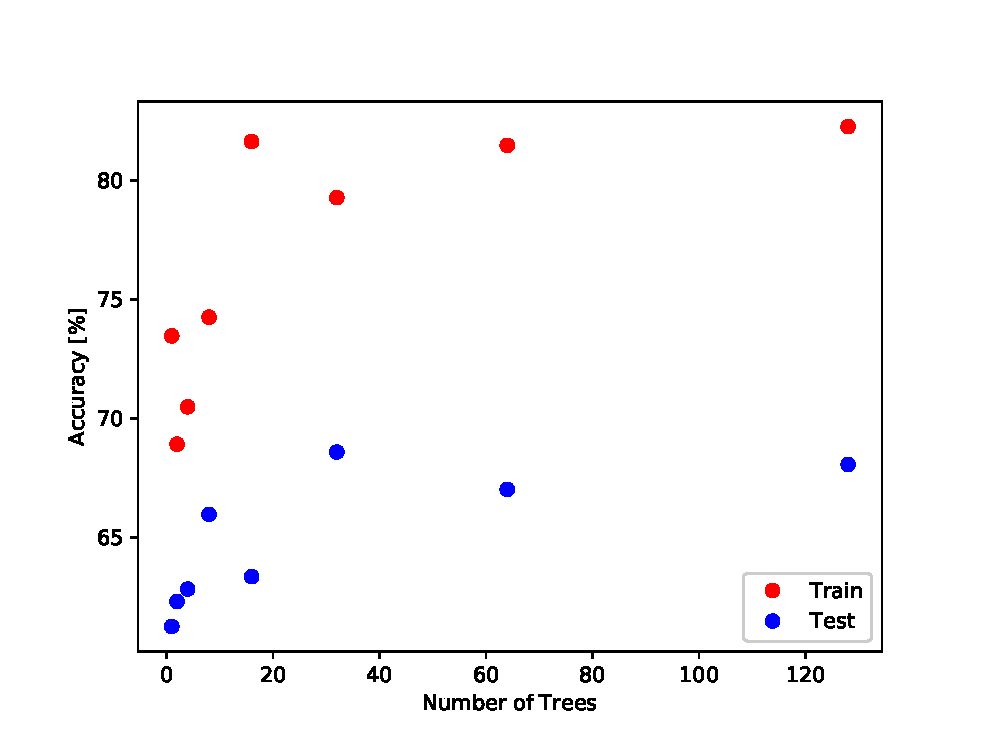
\includegraphics[scale=0.5]{n_trees}
%\framebox[4.0in]{$\;$}
%\fbox{\rule[-.5cm]{0cm}{4cm} \rule[-.5cm]{4cm}{0cm}}
\end{center}
\caption{Showing Random forest inhibition to produce over fitting errors even with increased complexity by large number of trees.}
\label{fig:n_trees}
\end{figure}

The ability of Random forests to resist over fitting is largely due to the number of trees and features, which is demonstrated in figure ~\ref{fig:n_trees}. Randomization increases bias but makes it possible to reduce the variance of the corresponding ensemble model through averaging. \cite{formann-roe_2012} It has been shown however that by increasing the maximum depth of each tree, a level of over fitting can be present, and similarly, that having shallow trees can produce low-confidence predictions. \cite{Criminisi2011} It is thus important that an appropriate value of the maximum depth be used, as its optimal value is related to the problem complexity. We investigated the depth of trees on accuracy, shown in figure ~\ref{fig:max_depth} below. We notice a small decrease in the accuracy at 20 features, and therefore choose an optimal at 15. This demonstrates that Random forests are still susceptible to over fitting, albeit less sensitive than many other machine learning algorithms without active regularization.

\begin{figure}[h]
\begin{center}
%\AddToShipoutPicture see eso-pic
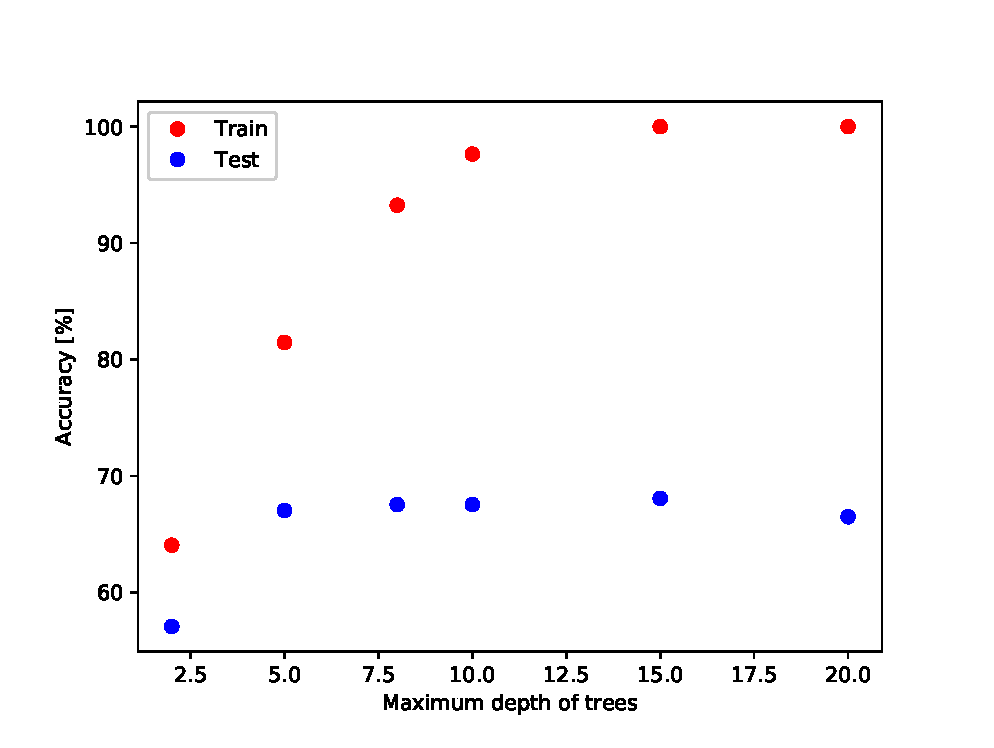
\includegraphics[scale=0.5]{max_depth}
%\framebox[4.0in]{$\;$}
%\fbox{\rule[-.5cm]{0cm}{4cm} \rule[-.5cm]{4cm}{0cm}}
\end{center}
\caption{Showing accuracy of Random forest with 64 trees with varying maximum depth of each decision tree. It should be noted that there is a slight decrease in the test accuracy at 20 features which can possibly be related to over fitting on the training data which reaches 100\% after 15.}
\label{fig:max_depth}
\end{figure}

\begin{figure}[h]
\begin{center}
%\AddToShipoutPicture see eso-pic
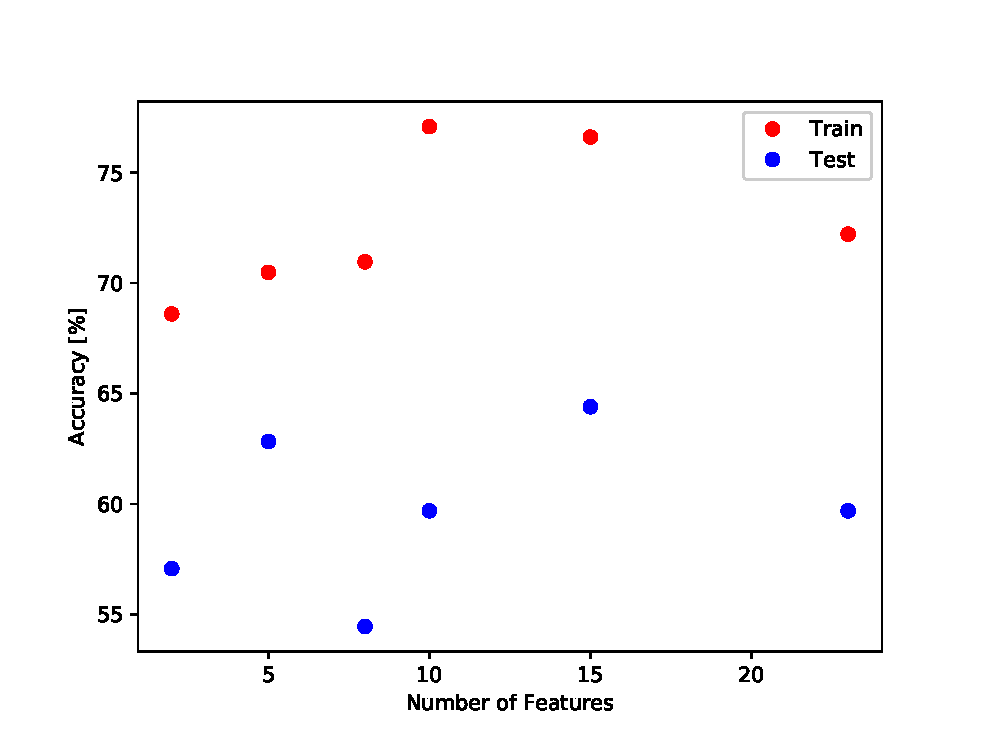
\includegraphics[scale=0.5]{n_features}
%\framebox[4.0in]{$\;$}
%\fbox{\rule[-.5cm]{0cm}{4cm} \rule[-.5cm]{4cm}{0cm}}
\end{center}
\caption{Showing the impact of the number of features used when constructing decision trees in Random forest with 64 trees and max depth 5. The optimal for testing is shown to be 5, which also agrees with literature on square-root of number of features}
\label{fig:n_features}
\end{figure}



%Can't get it to center this table...
\begin{table}[t]
\caption{Optimal values found for sci-kit learn Random forest by grid search}
\begin{center}
\begin{tabular}{cccccc}
{\bf Target class} &{\bf Max depth} &{\bf Num features} &{\bf Min samples per leaf} &{\bf Min samples for split} &{\bf Num of trees}
\\ \hline \\
GP\_greater\_than\_0         &8	&5	&2	&2	&128 \\
sum\_7yr\_GP         &8	&5	&4	&2	&64 \\
\label{scikit-table}
\end{tabular}
\end{center}
\end{table}


\begin{table}[t]
\caption{Comparison of Random forest classifier for GP\_greater\_than\_0}
\label{clas-table}
\begin{center}
\begin{tabular}{lll}
\multicolumn{1}{c}{\bf Machine Learning Package} &\multicolumn{1}{c}{\bf Accuracy} &\multicolumn{1}{c}{\bf Time}
\\ \hline \\
Weka         &69.4\%	&$<$1sec \\
scikit-learn             &70.7\%	&TIME \\
our implementation             &68.6\%	&$\approx$ 3min \\

\end{tabular}
\end{center}
\end{table}

From Table~\ref{clas-table}, it can be seen that all three implementations of Random forest yield similar results. It was noted however that when performing on standardized data so values are centered by their means and divided by the standard deviation, the accuracy was significantly lower for all three implementations, around 55\% accuracy. This can be due to the sensitivity of the splitting using gini impurity or entropy with small values, or perhaps some information is lost on the impact of certain features. The time taken for completion is difficult to compare since coding implementations are different, however using 4 workers running using the same parameters as shown in table ~\ref{scikit-table} the time of 3 minutes is slow, however not unreasonable. 

TODO: Figure out if this paragraph should be removed.
Random forests have been shown to achieve high classification performance through ensemble with a set of decision trees that are constructed using randomly selected feature subspaces. The performance of an ensemble learner is dependent on the accuracy of each component learner and the diversity of the components, especially when using a small set of trees which may be limited due to computational cost. The randomization can cause occurrence of bad predicting trees as well as correlated trees which can lead to poor ensemble decisions, which can be observed when performing multiple training runs using the same parameters which can lead to different accuracy results. Attempts have been made to improve the performance of this model by building a forest of only uncorrelated high performing trees. \cite{Bharathidason2014}

\section{Conclusion}
TODO: Summarize our findings and mention future work which is the uncorrelated tree algorithm in the paper I found before.


\subsubsection*{Contributions}
All authors contributed equally.\\
See GitLab repository here for specific commits:\\
\href{
    https://csil-git1.cs.surrey.sfu.ca/rkm3/mlclass-1777-randomforest
}{
    https://csil-git1.cs.surrey.sfu.ca/rkm3/mlclass-1777-randomforest
}


\small{
\bibliography{report}
\bibliographystyle{ieeetr}
}

\end{document}
